\noindent

\includegraphics[height=1.25cm]{images/pictograms/replication}
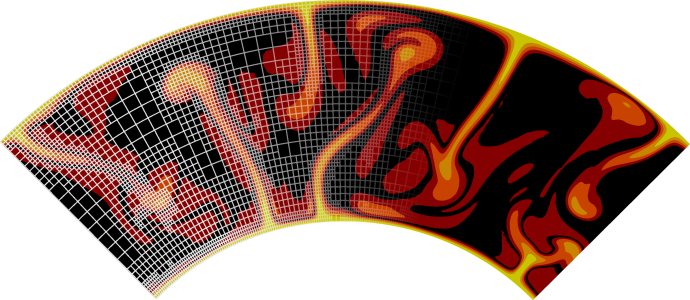
\includegraphics[height=1.25cm]{images/pictograms/aspect_logo}

\includegraphics[height=1.25cm]{images/pictograms/benchmark}

\includegraphics[height=1.25cm]{images/pictograms/under_construction}

\includegraphics[height=1.25cm]{images/pictograms/FEM}

\includegraphics[height=1.25cm]{images/pictograms/paraview}

%%%%%%%%%%%%%%%%%%%%%%%%%%%%%%%%%%%%%%%%%%%%%%%%%%%%%%%%%%%%%%%%%%%%%%%%%%%%%%%%%%%%%%%%%%%%%%%%%%%

\begin{flushright} {\tiny {\color{gray} python\_codes/fieldstone\_160/text.tex}} \end{flushright}

%\lstinputlisting[language=bash,basicstyle=\small]{python_codes/template_keywords.key}

\par\noindent\rule{\textwidth}{0.4pt}

\begin{center}
\inpython
{\small Code: \url{https://github.com/cedrict/fieldstone/tree/master/python_codes/fieldstone_160}}
\end{center}

\par\noindent\rule{\textwidth}{0.4pt}

{\sl This stone was developed in collaboration with J.C. Afonso}. \index{contributors}{J.C. Afonso}

\par\noindent\rule{\textwidth}{0.4pt}


%%%%%%%%%%%%%%%%%%%%%%%%%%%%%%%%%%%%%%%%%%%%%%%%%%%%%%%%%%%%%%%%%%%%%%%%%%%%%%%%%%%%%%%%%%%%%%%%%%%


There are three materials in the domain:
\begin{itemize}
\item crust: $\rho_{crust}=2300~\si{\kg\per\cubic\meter}$ and $\eta_{crust}=10^{23}~\si{\pascal\second}$;
\item mantle: $\rho_{mantle}=3300~\si{\kg\per\cubic\meter}$ and $\eta_{crust}=10^{21}~\si{\pascal\second}$;
\item weak zones: $\rho_{wz}=\rho_{crust}$ and $\eta_{wz}=10^{-3}\eta_{crust}$.
\end{itemize}
The domain is a Cartesian box of size $L_x=120~\si{\km}$, $L_y=100~\si{\km}$.
Free slip boundary conditions are imposed on all four sides. ${\bm Q}_2 \times Q_1$ elements are used.
The crust is 20~\si{\km} thick but is thickened (40~\si{\km} depth) in the middle 30~\si{\km}.
On each side we find weak zones as thick as the crust and 1~\si{\km} wide. 
The default resolution is set to 120$\times$1200 elements.

Pressure normalisation?

























%%%%%%%%%%%%%%%%%%%%%%%%%%%%%%%%%%%%%%%%%%%%%%%%%%%%%%%%%%%%%%%%%%%%%%%%%%%%%%%%%%%%%%%%%%%%%%%%%%%
\par\noindent\rule{\textwidth}{0.4pt}

\vspace{.5cm}

\begin{center}
\fbox{\begin{minipage}{0.9\textwidth}
{\color{teal}To Do, open questions, future work?}
\begin{itemize}
\item do smthg
\end{itemize}
\end{minipage}}
\end{center}

%%%%%%%%%%%%%%%%%%%%%%%%%%%%%%%%%%%%%%%%%%%%%%%%%%%%%%%%%%%%%%%%%%%%%%%%%%%%%%%%%%%%%%%%%%%%%%%%%%%
\vspace{.5cm}

\Literature:\\
\fullcite{xxxxYY}


